\documentclass[hidelinks, 12pt,letterpaper]{article}
%%%%%%%%%%%%%%%%%%%%%%%%%%%%%%%%%%%%%%%%%%%%%%%%%%%%%%%%%%%%%%%%%%%%%%%%%%%%%%%%%%%%%%%%%%%%%%%%%%%%%%%%%%%%%%%%%%%%%%%%%%%%
\usepackage{amsmath}
%\usepackage{graphicx,fancyheadings}
\usepackage{fancyhdr}
\pagestyle{fancy}
\usepackage{graphics}
\usepackage{amssymb}
\usepackage{verbatim}
\usepackage{setspace}
\usepackage{ulem}

\usepackage{amssymb}
\usepackage{graphicx}
\usepackage{amsmath}
\usepackage{verbatim}
\usepackage{setspace}
\usepackage{ulem}
\usepackage{textpos}
\usepackage{changepage}
\usepackage{url}
\usepackage{hyperref}

\usepackage{color}
\usepackage{xcolor}
 

%\renewcommand{\sout}[1]{}
%\renewcommand{\bf}{}

\usepackage[round]{natbib}
% \usepackage[backend=biber,style=apa,autocite=inline]{biblatex} \DeclareLanguageMapping{english}{english-apa}
% \addbibresource{./sshrc2023shipping.bib}


%\lhead{} \chead{} \cfoot{}
\renewcommand{\headrulewidth}{0pt}
\renewcommand{\footrulewidth}{0pt}
\renewcommand{\baselinestretch}{1.1}
%\textheight 8in \textwidth 6in \oddsidemargin 0.15in
%\evensidemargin 0in \headheight 14.5pt \headwidth 6in \parskip 4pt

\pagestyle {empty}

\setlength{\topmargin}{0.0cm} \setlength{\headheight}{0cm}
\setlength{\headsep}{0.3cm} \setlength{\topskip}{0cm}
\setlength{\textheight}{22.5cm} \setlength{\textwidth}{16.6cm}
\setlength{\oddsidemargin}{0cm} \setlength{\evensidemargin}{0cm}
\setlength{\footskip}{0.5cm}
\newcommand{\indep}{\perp \!\!\! \perp}


\newcommand{\Red}{\color{red}}
\newcommand{\Blue}{\color{blue}}
\newcommand{\ve}{\varepsilon}

\def\bs{\boldsymbol}

%\setlength{\topmargin}{-0.2cm} \setlength{\headheight}{0cm}
%\setlength{\headsep}{0.3cm} \setlength{\topskip}{0cm}
%\setlength{\textheight}{22cm} \setlength{\textwidth}{16.2cm}
%\setlength{\oddsidemargin}{0cm} \setlength{\evensidemargin}{0cm}
%\setlength{\footskip}{1cm}

\usepackage[letterpaper]{geometry}

\usepackage{graphicx}
\graphicspath{{../images/shared/}}


 \rhead{Hiroyuki Kasahara \hspace{-1.7cm} }
 %\lfoot{}
 \cfoot{\thepage \hspace{-2cm}}



%\setcounter{page}{10}

\begin{document}
\bibliographystyle{asa}

% Challenge—The aim and importance of the endeavour (40\%):
% \begin{itemize}
%   \item originality, significance and expected contribution to knowledge;
%   \item appropriateness of the literature review;
%   \item appropriateness of the theoretical approach or framework;
%   \item appropriateness of the methods/approach;
%   \item quality of training and mentoring to be provided to students, emerging scholars and other highly qualified personnel, and opportunities for them to contribute; and
%   \item potential for the project results to have influence and impact within and/or beyond the social sciences and humanities research community.
% \end{itemize}

% Feasibility—The plan to achieve excellence (20\%):
% \begin{itemize}
%   \item appropriateness of the proposed timeline, and probability that the objectives will be met;
% \end{itemize}

\begin{center}
\textbf{Detailed Description of Proposed Research: }\vspace{-0.25cm}
\end{center}

\noindent \textbf{Project: Quantifying the response of maritime shipping CO$_2$ emissions to economic shocks and policy regulations}
\smallskip

\noindent \textbf{Objective:} First, we quantify weekly, fleet-level CO$_2$ emissions from worldwide maritime shipping activity before and during the COVID pandemic.
Second, we examine the change in CO$_2$ emissions from maritime shipping during the COVID pandemic in terms of changes in bilateral trade volumes and provide a decomposition analysis. 
%¬ a bit confusing, wording not quite right
Third, we estimate the heterogenous elasticities of CO$_2$ emissions from maritime shipping with respect to international trade using the COVID pandemic demand shock as a source of significant variation, which in turn is used for conducting a counterfactual analysis of implemeting policy regulations.
%¬ come back to this
\smallskip

\noindent \textbf{Context:} 
Global trade is intricately linked with maritime shipping, which transports over 80\% of the volume of all traded goods and around 70\% of their value \citep{unctad2017review}.
% The importance of the shipping industry has become particularly apparent in recent years as disruptions ranging from the blockage of the Suez Canal to widespread COVID-related port slowdowns have snarled supply chains world-wide.
At the same time, maritime shipping contributes \textcolor{blue}{one-third of CO$_2$ emissions from all trade-related activities (source), which corresponds to}
about 3\% of global CO$_2$ emissions, roughly equal to the total emissions of Germany \citep{faber2020fourth}. The International Maritime Organization (IMO) has set a target of a 50\% reduction by 2050 and has introduced a minimum efficiency requirement for new ships in 2013, with stringency increasing over time and future levels yet to be determined.    %\textcolor{blue}{mention difficulty of decarbonization?}
The stringency of abatement actions required to meet this goal clearly depends on how trade will evolve over the coming decades, and a thorough understanding of this relationship is essential for effective policy.  %A continuation of the trend of increasing trade would make this goal much more difficult to hit. Faced with this uncertainty, the IMO and its consituent countries are developing and implementing policies to reduce shipping emissions, with new efficiency regulations being phased in this year. 



%TOPIC: Analyze change in emissions and trade during COVID
%Trade volumes fluctuated substantially during the COVID pandemic:
While trade volumes typically vary slowly, the COVID pandemic induced substantial variation over a short period:
World merchandise trade decreased by more than 10 percent in the first three months of the pandemic before recovering over the following two years \citep{oecd21}. %Furthermore, the extent to which trade decreased differ across countries and industries.  
We first measure the change in shipping emissions before and during this period using high-frequency data of ships' movements, which we then relate to the change in bilateral trade volumes between country pairs. By exploiting the large variation in shipping, we estimate the short- to medium-run elasticity of CO$_2$ emissions from maritime shipping with respect to international trade. In doing so, we provide an
% a quantitative analysis of how a change in trade volumes affects CO$_2$ emissions from maritime shipping, providing 
important quantitative analysis to inform policymakers in assessing the effectiveness of emissions regulations.  %We then use the estimated elasticities to compute how a change in trade volumes before and during/after the COVID pandemic led to a change in CO$_2$ emission from maritime shipping across different country pairs, as well as, by aggregate, in the entire world. 

%TOPIC: Dynamic, more causal relation for counterfactuals
% How much did the CO$_2$ emission from maritime shipping decline due to the contraction of world trade in the midst of the COVID pandemic? Quantifying the elasticity of CO$_2$ emissions with respect to trade volumes is important for predicting how an increase in international trade affects CO$_2$ emissions in future. 
Quantifying the elasticity of shipping emissions to trade is challenging for a number of reasons. A ship's fuel consumption depends on many factors, including its size and age, with newer and larger ships typically more efficient. The existing fleet is extremely heterogeneous: \autoref{fig:distribution} illustrates the large variation across both dimensions in just a subset of ships, namely small to medium bulk carriers (This excludes the largest class up to 400'000 deadweight tonnes (DWT)). Furthermore, new ships have become larger over time. Ship size is related to the volume of trade, the type of products shipped, and port and canal infrastructure. As such, different bilateral trade relationships involve different sizes of ships and hence different fuel efficiency, leading to heterogenous emissions--trade elasticity across different country pairs. In addition, the presence of trade imbalances means ships often travel without cargo on certain routes. Finally, fuel consumption depends roughly cubicly on speed, meaning that the short-run elasticity of emissions to shipping demand may be quite large and may fluctuate over time with the price of fuel. 
% making it complicated to estimate the relationship between fuel consumption and trade volumes from the data on ship movements.
% As such, ships adapt differently and which ships change speed or idle is important for determining overall emissions.  

\begin{figure}[h]
  \centering
  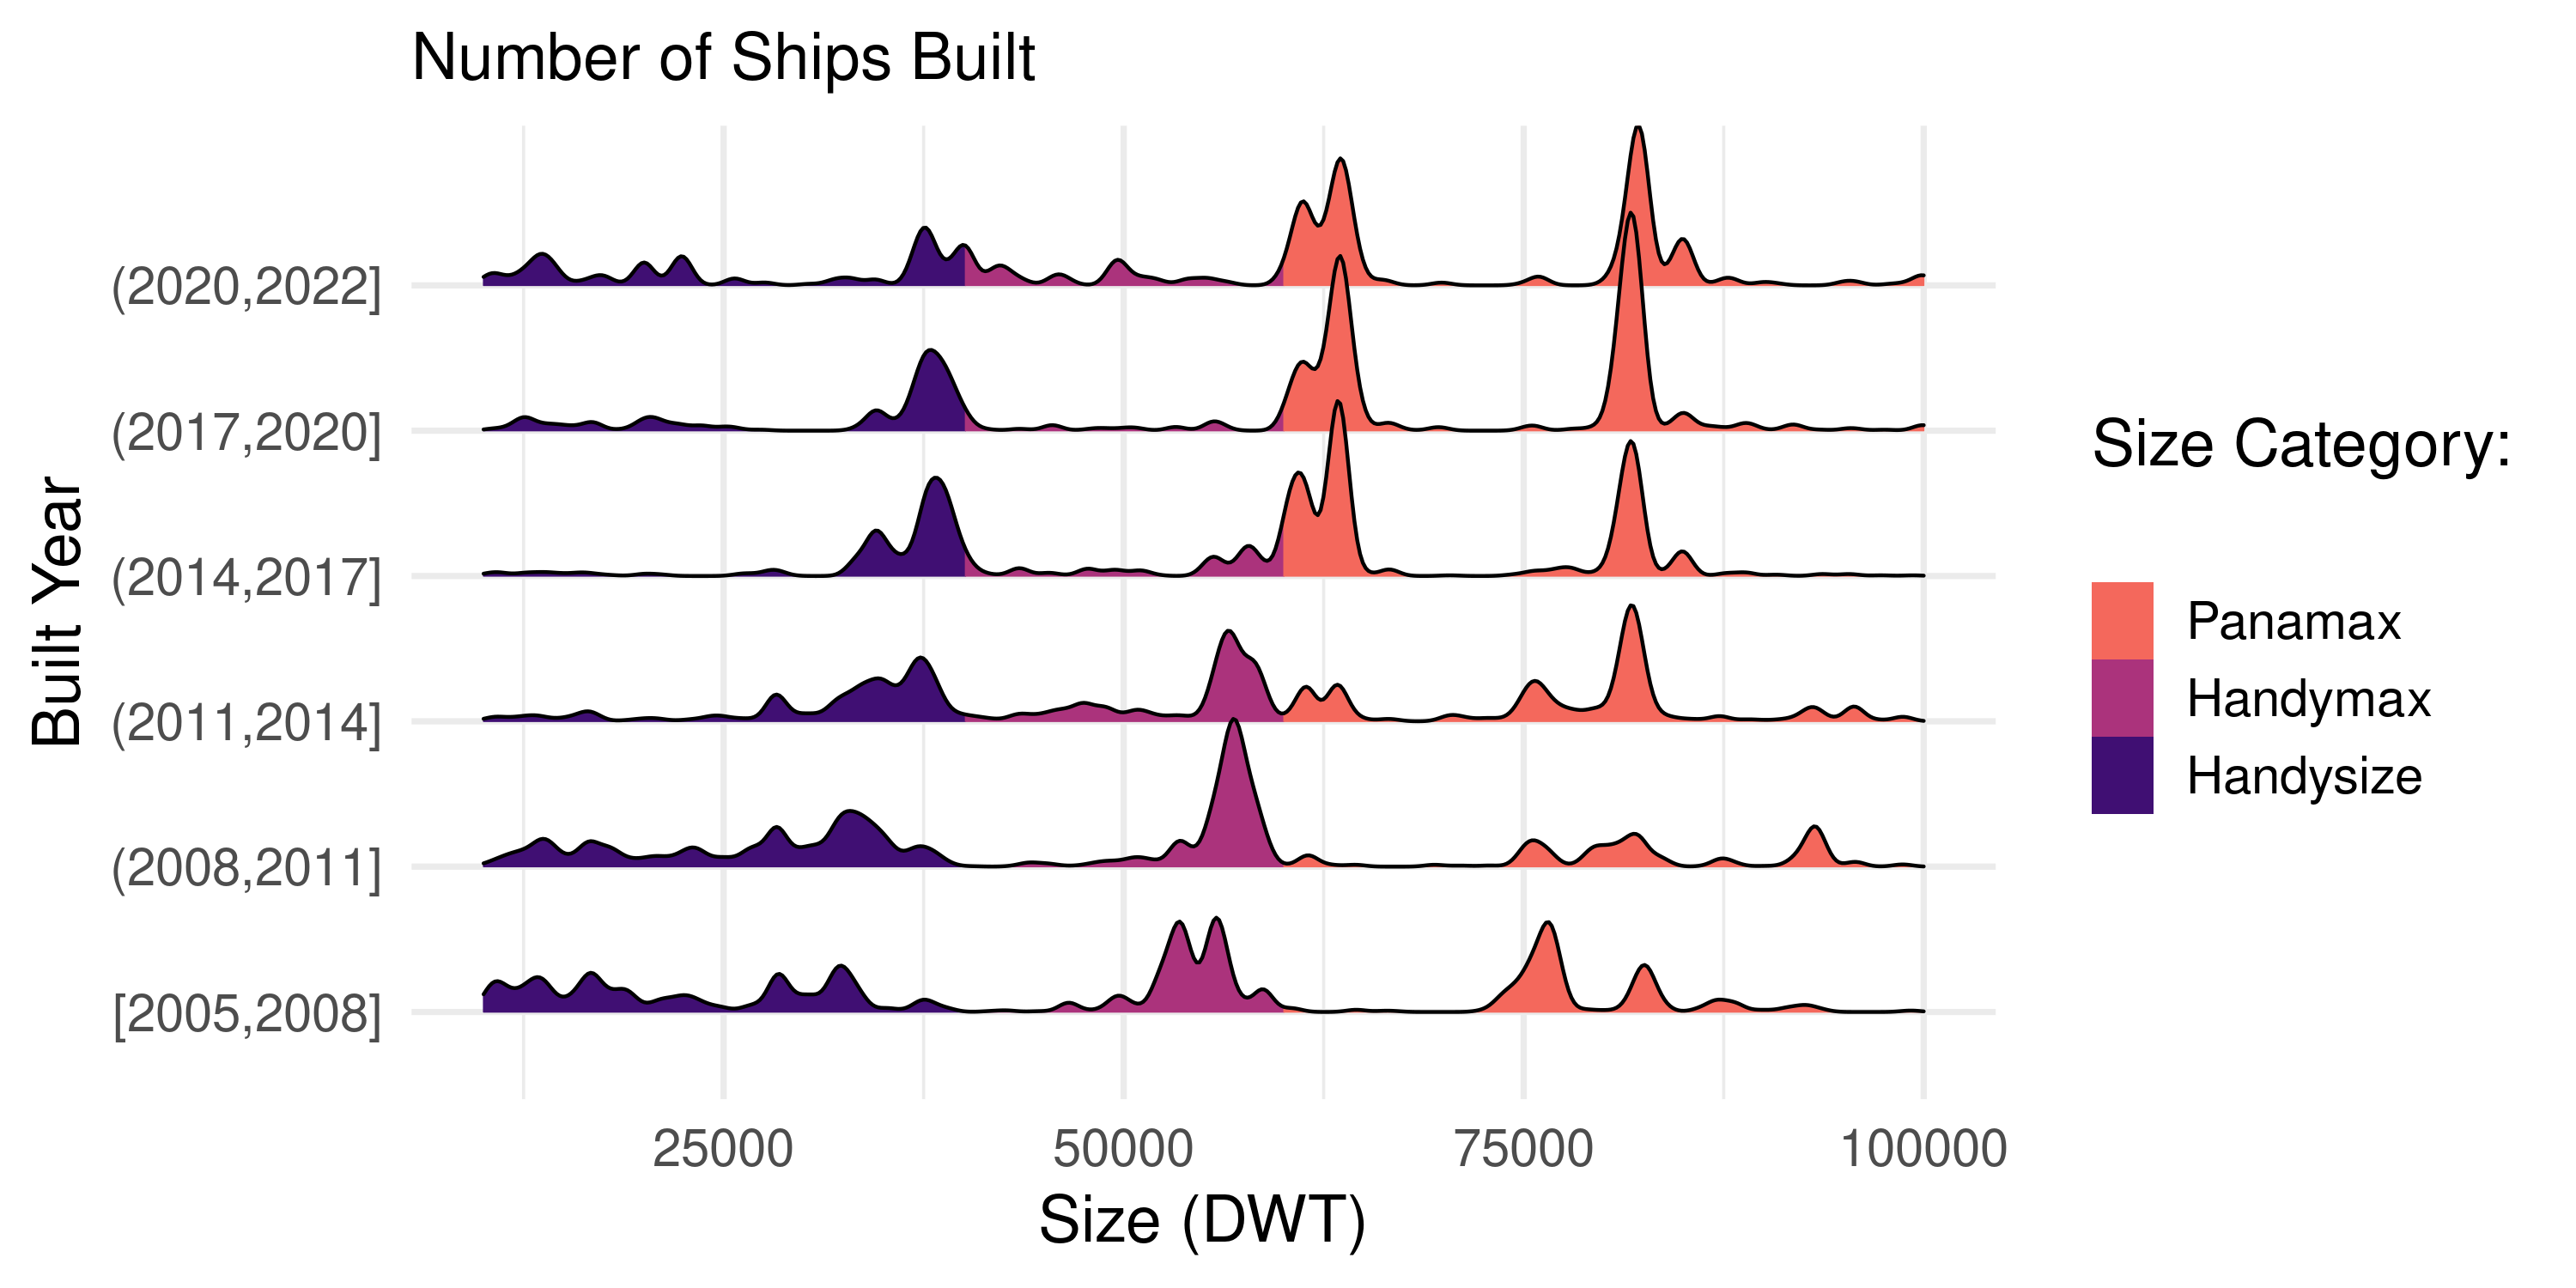
\includegraphics[width = 0.6\textwidth]{WFR_Bulkers_Exploration_Size_Built_horizontalridges.png}
  \caption{Existing fleet of bulk carriers by size and built year.}
  \label{fig:distribution}
\end{figure} 
%We use  the detailed high-frequency satellite data of ships' movements merged with the data on ship characteristics as well as the data on annual fuel consumption for EU ships to estimate how fuel efficiency depends on age, speed, size, the level of draft (which measures the capacity utilizations), and other ship characteristics. 

 
 
%
%The three largest sectors of maritime shipping, jointly accounting for over half of maritime emissions, are containerships, bulk carriers, and tankers. These ships transport, respectively,  containerized goods (often manufactured goods), dry bulk goods (e.g. coal, ores, grains), and bulk liquids (primarily oil). As such, they contribute to diverse links of the overall supply chain and are impacted differently by fluctuations in trade. Furthermore, each sector has distinct market characteristics. For example, containerships typically operate with fixed routes and schedules, while bulk carriers tend to operate much more flexibly. Ownership structures reflect these differences as well, with the containership sector being highly concentrated and the bulk carrier sector highly \textit{un}concentrated.
%
%Despite their differences, the various sectors share some common mechanisms by which they adjust to demand. Because new ships cost tens to hundreds of millions of dollars, last for over 25 years, and take two to five years to build, adjustments in fleet capacity are slow to occur. On shorter time horizons, shipping supply adjusts to changing levels of demand primarily through a combination of changing travel speed and temporarily idling ships, though quantifying these adjustments is an active area of research (see \citet*{adland2018dynamic, ollila2022effect,assmann2015missing}). 

%The IMO has introduced three separate emissions regulations. The first, implemented in 2013, is a minimum efficiency requirement for new ships, with stringency increasing over time and future levels yet to be determined. As of the beginning of 2023, a similar regulation now applies to all existing ships and an additional regulation has be added that requires operational efficiency of each ship to be continuously improved moving forward. %Uncertainty surrounding these regulations, as well as future technological developments has led to reduced new ship building activity in the past years. With a diminished extrinsic margin for adjustment in addition to the already slow natural fleet development, this places further importance on quantifying the intrinsic margin for predicting the path of shipping emissions.

%TOPIC: Relation to emissions estimates in lit.
The most extensive existing literature quantifying shipping emissions comes from the IMO itself, in cooperation with a handful of related organizations: The Fourth IMO GHG Study 2020 \citep{faber2020fourth} details both bottom-up and top-down methodologies for calculating emissions. Their bottom-up approach employs data collected from ships' automatic identification systems (AIS) which transmit the location and speed of each ship every few minutes. This approach has been developed by various authors, including \citet{jalkanen2009modelling}, \citet{olmer2017greenhouse}, and \citet{johansson2017global}. In order to estimate CO$_2$ emissions, they combine AIS data with ship fuel consumption ratings and aggregate. Our approach is similar, but leverages actual emissions reports to estimate fuel efficiencies.

%TOPIC: Relation to trade/shipping lit.
A small number of authors have explored the relation between trade and shipping. \citet{cristea2013trade} and \citet{shapiro2016trade} take macroeconomic approaches to look broadly at emissions from all transporation modes invovled in trade. Focusing on maritime shipping, \citet{van2018spatially} and \citet{liu2019emissions} link AIS data with granular indicators of trade volumes to create region-specific estimates. Most closely related to our work, \citet{wang2021trade} calculate bilateral seaborne trade volumes and link them with shipping emissions estimated from AIS data. They provide a snapshot of values for the year 2018 and develop a model based on nominal efficiencies for exploring counterfactuals. With a more empirical approach \citet{brancaccio2018impact} explore the elasticity of trade with respect to ship fuel costs. Our work will be among the first to seriously explore the relationship in the opposite direction --- from trade to emissions --- on a global scale. We borrow from the methods of \citet{wang2021trade}, but we propose a novel empirical method to estimate efficiencies using reported fuel consumption from the European Union's (EU) Monitoring, Reporting, and Verification (MRV) program. Furthermore, we leverage COVID-related variations to calibrate and validate our model. The use of actual reported emissions allows us to capture more of the previously discussed adjustment channels, and the large cross-sectional/time-series variation in shipping activity during the COVID pandemic aids identification. %We hope to provide important quantitative estimates to help inform policy makers in assessing the effectiveness of emissions regulations and setting their stringency levels going forward. 

 \smallskip

%TOPIC: Overview
\noindent \textbf{Methodology:}  We first estimate how a ship's fuel consumption efficiency is determined by ship's speed, location, draft, and ship's observed characteristics. Then we compute high-frequency emissions estimates for each ship's voyages between ports. This first stage relies on three key datasets that we have obtained: (i) AIS tracking data, (ii) the World Fleet Register, and (iii) the MRV data.

%TOPIC: Shipping data description
We have obtained hourly AIS tracking data for the entire fleets of bulk carriers and containerships from the beginning of 2019 to the end of 2021. This includes information on speed, location, and draft (the vertical distance between the waterline and the bottom of the hull), which can be used to determine whether a ship is carrying cargo or not. We match this data to the World Fleet Register from Clarksons Research, which is a virtually complete listing of all large merchant ships that includes basic  information on each ship, including built year, size, and type, and for many ships includes highly detailed technical characteristics such as hull dimensions, engine power, propeller details, etcetera. Finally, we further link this to publicly available data from the EU's MRV regulation, which provides annual fuel consumption and emissions for trips into and out of the EU (``EU trips,'' hereafter). This data begins in 2018 and naturally includes only ships with portcalls in the EU.

%TOPIC: Detail efficiency estimation
Our methodology for estimating fuel efficiency builds on that of the IMO as detailed in \citet{faber2020fourth}.
% and follows closely the data cleaning and matching procedures described therein.
However, whereas they use theoretical fuel consumption values corresponding to rather coarse ship size- and age-bins, we empirically estimate ship-specific fuel efficiencies using actual fuel consumption data and all available ship characteristics. 
% In particular, we use actual fuel consumption data  from the MVR data while  \citet{faber2020fourth} does not use any fuel consumption data  by themselves--- rather, fuel consumption is computed using pre-determined formula based on theoretical assumption on specific types of ships. By using actual fuel consumption data, we hope to better estimate how fuel consumption is determined under actual operating conditions. 

Our procedure is as follows. First, we identify trips from the AIS data as between two stops of a sufficient length in proximity to land, and flag EU trips as those with at least one stop within the EU. To ensure the accuracy of our data, we use data only for ship-year observations for which the total distance of detected trips to/from the EU agrees closely with the distance reported in the MRV data. %With this travel history constructed, we calculate a proxy for the travel work performed by a ship in a given year as the sum of its speed squared multiplied by the distance travelled between every pair of observations in the AIS data. The fuel efficiency is then calculated as the reported annual fuel consumption divided by the inferred annual travel work.
Next, we estimate how fuel efficiency, accounting for the detected EU trip operating conditions (speed, draft), is determined by ship characteristics (age, size, etc.) using the fuel consumption data for EU trips from the MRV dataset. 
Then, we extrapolate these efficiencies to non-reporting ships --- ships that did not stop at an EU port --- based on their operating conditions and ship characteristics. 
% Given ship efficiencies, we can calculate a monthly emission estimate for each ship. 
These estimates can be aggregated at any desired level. To our knowledge, this will be the first work to employ the MRV data to estimate fuel efficiency. \citet{uge2020estimation} also link MRV data with AIS data, but they use it in the opposite sense---to validate reported emissions in the MRV.

%TOPIC: Demonstrate feasibility, utility, progress
As a preliminary investigation, we have estimated fuel efficiencies for bulk carriers, regressing fuel efficiency on a set of ship characteristics (using logs of all variables) as well as built-year fixed effects.
 \begin{equation}\label{eq1}
 \log\left(
     \frac{fuel~consumption}{size \cdot \sum_{x \in X}  \cdot s_x^2 \cdot x}
 \right)_{it}
         = built~year_{i} + \boldsymbol{\beta} f(Z_i) + \varepsilon_{it},
 \end{equation}
 where $fuel~consumption$ is reported annual consumption, $size$ is the ship's capacity in deadweight tonnage, $x$ is the distance travelled at each speed $s_x$, $Z_i$ is a vector of ship's characteristics (including $size$), and $f(\cdot)$ is an unknown function, which we use semi-parametric sieve methods using B-splines as well as machine learning tools (e.g., random forest, deep neural network) to estimate.
 
 \begin{figure}[h]
  \centering 
  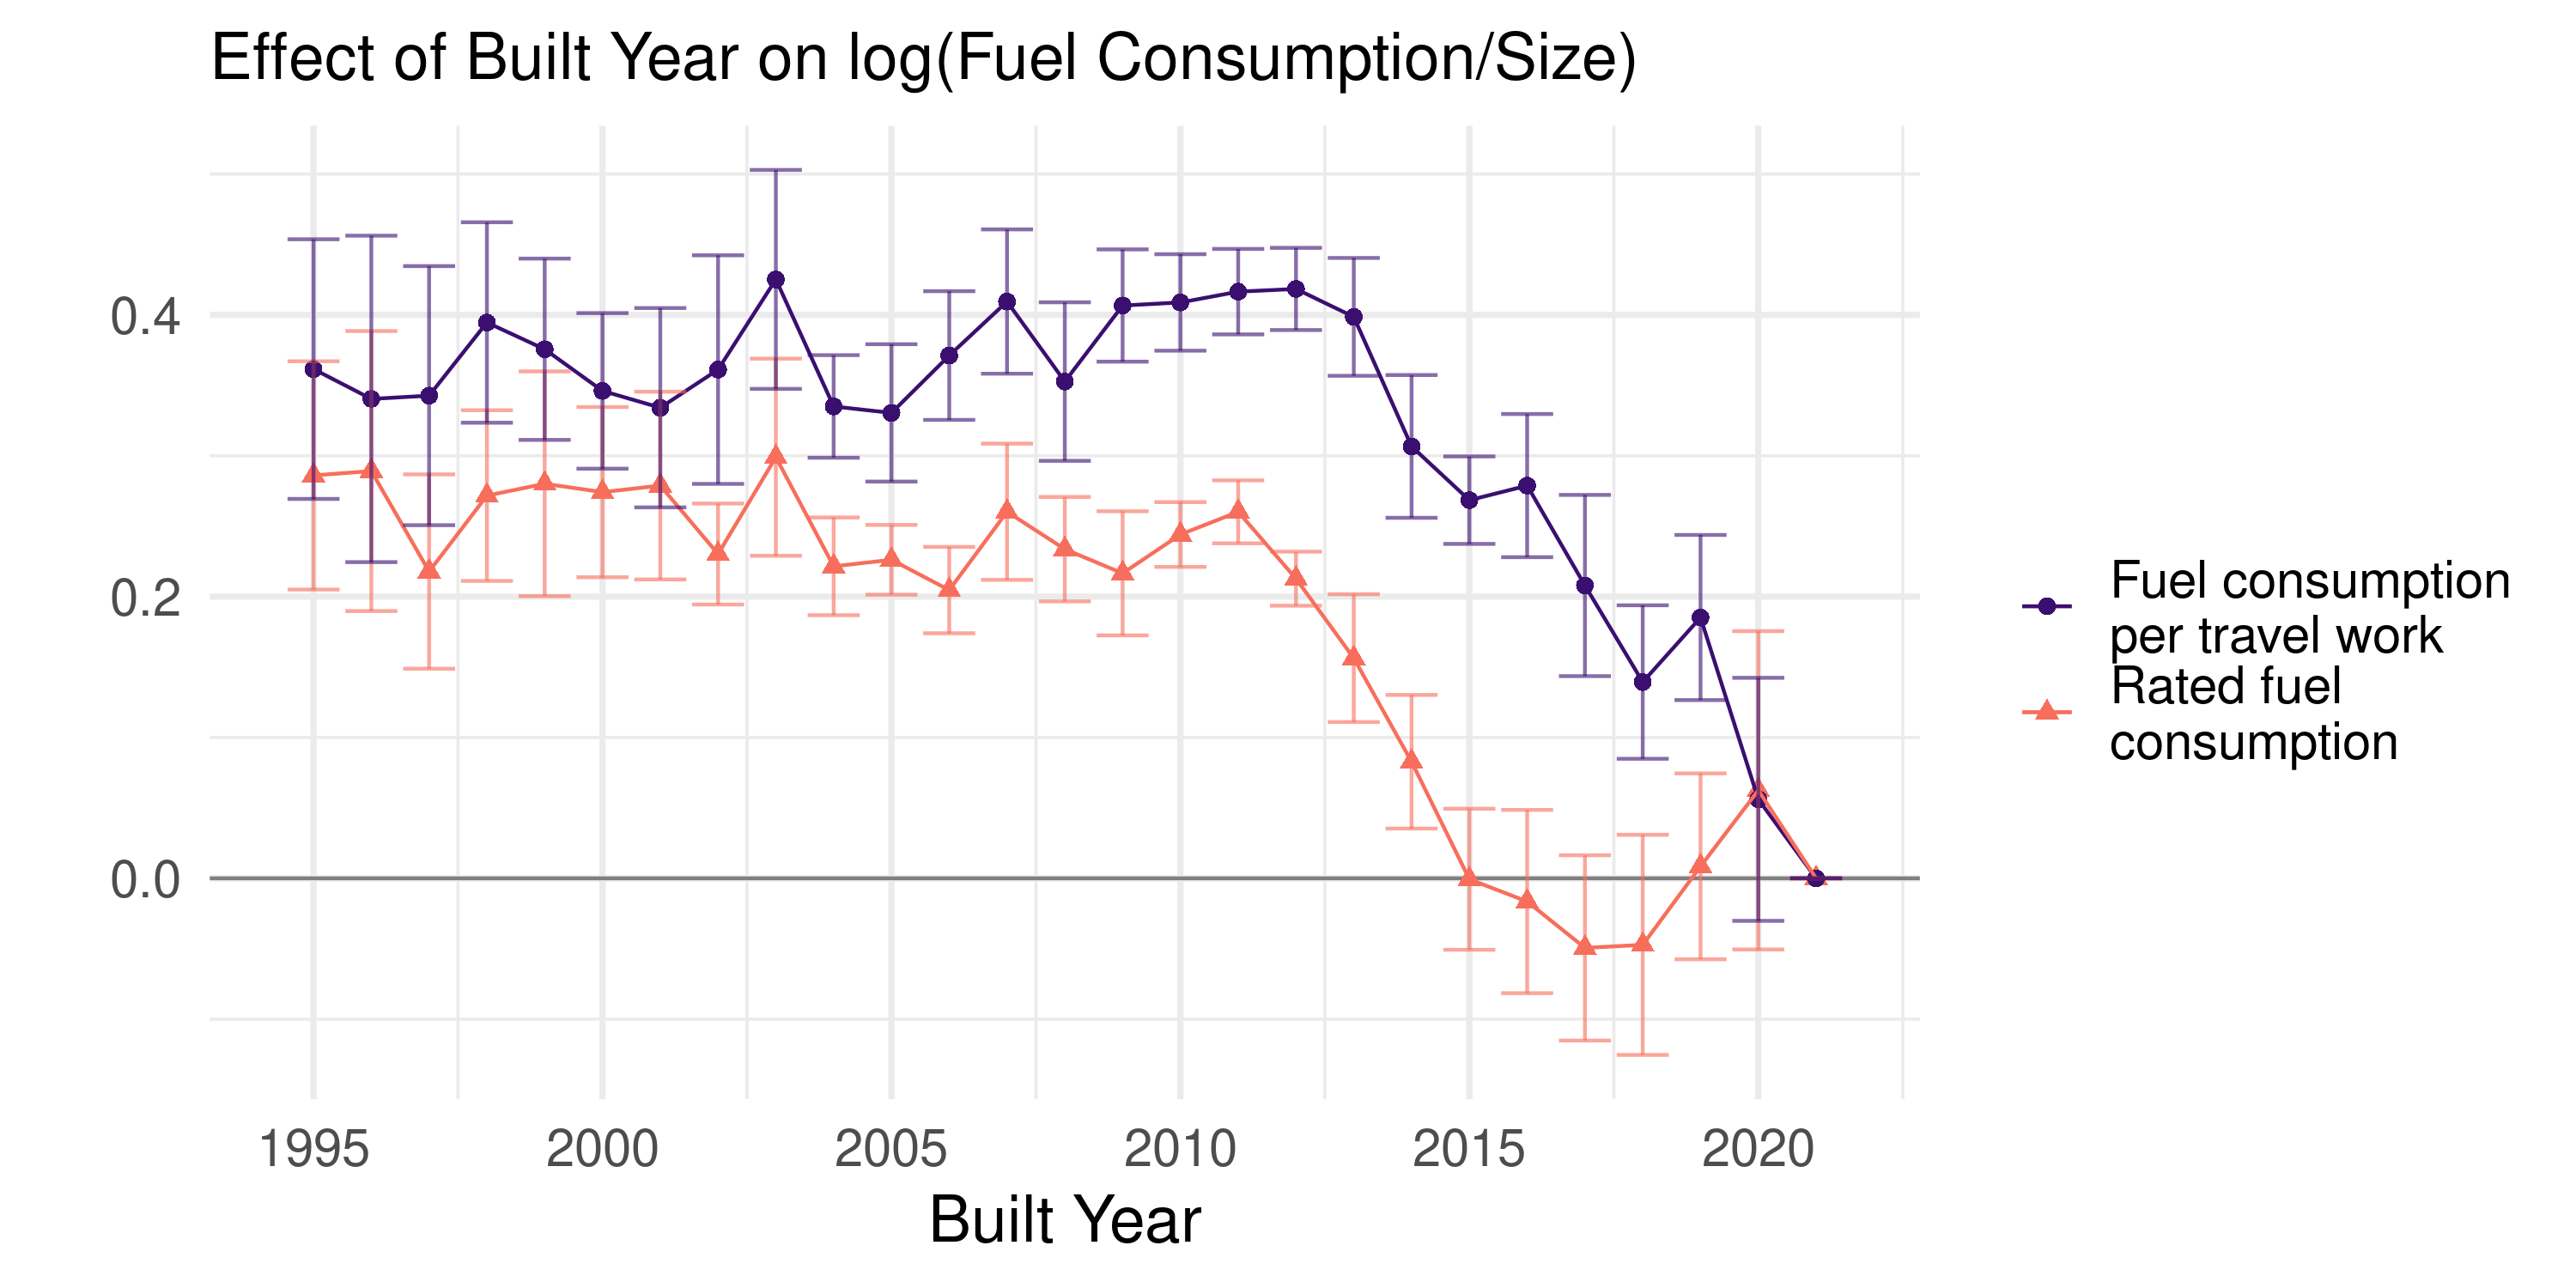
\includegraphics[width = 0.6\textwidth]{Efficiency_Regression_Size_Built_coefs_1and3_ggplot.png}
  \caption{Built year fixed effects from efficiency regression (\ref{eq1}). Error bars represent 95\% confidence intervals, with errors clustered at the individual ship level.}
  \label{fig:efficiency}
\end{figure} 

 \autoref{fig:efficiency} plots the built-year fixed effects for our preliminary estimation based on a log-linear specification. Efficiency is surprisingly flat for ships built before roughly 2013, after which it improved sharply. This agrees well with the analysis of evolution of new ship efficiency from \citet[][Figure 15]{faber2015historical}. We also include estimates using the rated, rather than the actual fuel consumption, which illustrates the difference between these approaches. The current specification does not include the effects of laden status or weather but we plan to include the draft level in the AIS data as well as wind/wave speeds using detailed weather data. % like that used by \citet{brancaccio2020geography}.  %As noted by \citet{olmer2017greenhouse}, details such as the engine power curve (how fuel consumption varies away from design speed), hull-roughening, and hull-fouling are hard to predict or attribute. 



%TOPIC: Why do differently?
A limitation of our proposed approach is that the fuel consumption data is annual and there may be significant error in calculating the travel work over such a long time period. On the other hand, the advantage with regards to the approach of \citet{faber2020fourth} is that it relies less on theoretical assumptions. For CO$_2$ emissions estimates, we plan to compare our estimate with that of \citet{faber2020fourth}. %Our estimates would incorporate these effects at the average level of observed ships

%TOPIC: Port to port level aggregation
Using the estimated fuel efficiency for each ship and its travel history, it is straightforward to compute the worldwide CO$_2$ emissions within each month of the years from 2017 to 2022 by aggregating fuel consumptions across all ships. This allows us to identify fuel consumption for each origin-port -- destination-port pair
% --- the fuel consumption associated with maritime shipping from port A to port B --- 
by aggregating all trips taken from port A to port B in each month. Further aggregating all ports within each country, we estimate the monthly CO$_2$ emissions associated with maritime shipping from each origin country to each destination country.
This allows us to analyze the source of a change in the worldwide CO$_2$ emission by decomposing it as the sum of a change in directional bilateral trade flows across different countries and directions. We emphasize the importance of directionality --- around 42\% of bulk carriers travel without cargo due to trade imbalances \citep{brancaccio2020geography} --- and account for it by identifying ship loading and unloading at each port using the level of draft from AIS data; for validation, we use the monthly  product-level  bilateral trade data  from UN Comtrade,
Eurostat, and the US census to examine how the directional trade volumes estimated by the AIS data corresponds to the reported  monthly bilateral trade volumes between two countries, where the proportion of seaborne trade is taken into account. 

%To date, we have estimated efficiencies using this procedure for bulk carriers. We have further constructed a simple linear predictive model for efficiency extrapolation, regressing fuel efficiency on a set of ship characteristics (using logs of all variables) as well as built-year fixed effects.
% \begin{equation}
% \log\left(
%     \frac{fuel~consumption}{Dwt \cdot \sum_{x \in X}  \cdot s_x^2 \cdot x}
% \right)_{it}
%         = \delta age_{it} + \boldsymbol{\beta}log(Z_i) + \varepsilon_{it}
% \end{equation}
%The coefficients for the built-year fixed effects are plotted in \autoref{fig:efficiency} and indicate that efficiency after controlling for size is surprisingly flat for ships built before roughly 2013, after which efficiency improved. This agrees qualitatively with the analysis of evolution of new ship efficiency from \citet{faber2015historical} (see Figure 15).

%TOPIC: Describe dynamic aspect (elasticity)
Finally, we model the elasticity of CO$_2$ emissions from maritime shipping with respect to the trade volume from origin country to destination country for any country pair that involves maritime shipping. The idea is that we estimate  the elasticity of CO$_2$ emissions specific to ship categories (type, size, age) and origin-desination pair and then compute the elasticity of CO$_2$ emissions with respect to trade volume from each origin country to each destination country by aggregating the elasticities across different ship categories using their  observed empirical shipping weights.

%TOPIC: Trade data and use
%\textcolor{blue}{Are we using actuall trade data or implied trade volumes from AIS? If former, describe trade data, seaborne trade calculation as per \citet{wang2021trade}, and use}

%TOPIC: Modelling details
Specifically, we create multiple categories of ships based on ship type (containerships, bulk carriers, and tankers), sizes, and ages. For each category, we estimate a version of the fuel efficiency equation (\ref{eq1}). As a benchmark, we evaluate the equation at the observed average speed and the average level of draft for each category of ships travelling from country A to B. This will allow us to compute the elasticity of fuel consumption (and CO$_2$ emission) with respect to an increase in trade volume shipped from country A to  B.  Note that these elasticities are different across ship categories; furthermore, it depends on the average speed and the average level of draft. The route-specific level of draft is also used to adjust the utilization of ship capacity to take into account of trade imbalance so that, for some ship route (e.g., shipping from China to Australia), the amount of traded goods shipped is much less than what the observed ship movements from China to Australia imply because many ships are near empty. 

%TOPIC: Where this is leading
The elasticity of  CO$_2$ emission with respect to trade volume depends on shipping speed, capacity utilization, and ship size. The required  fuel consumption and, hence, the CO$_2$ emission is less if the slower the speed, the higher the capacity utilization, and the larger the size of ships.  Using the estimated elasticities, we plan to evaluate the impact of implementing  the following two policy regulations on CO$_2$ emissions. First, we evaluate the effect of regulating the maximum speed of ships on CO$_2$ emissions. Second, we evaluate the effect of regulating unloaded trips in the context of trade imbalance. The proposed analysis has two important limitations. First,  our analysis abstract away from the general equilibrium effect \citep[e.g.,][]{shapiro2016trade}. Second, our project has limited scope in that we don't analyze the CO$_2$ emission from production of trade goods \citep[e.g.,][]{{cristea2013trade}}. Nonetheless, we hope that our analysis will provide an important stepping stone for future, more comprehensive quantitative analyses. 
%\textcolor{blue}{think about these counterfactuals}
%\textcolor{blue}{need to include mention of existing regulations if discussing regulation counterfactuals?}


 

% Trade
%% Data
%COVID variation
%\textbf{Trade data} Bilateral trade data from...
%
%\textbf{Method of linking to emissions to trade}
%Begin with global, then incorporate geographical variation
%
%
%\pagebreak
%Potential data purchases:
%\begin{itemize}
%  \item expand time series of AIS tracking data beyond 2021
%  \item AIS tracking data for tankers
%  \item bilateral trade
%\end{itemize}

\pagebreak

% \printbibliography[heading = subbibliography]
\singlespace{
\bibliography{sshrc2023shipping}
}



\end{document}
